\documentclass[tikz]{standalone}
\newcommand{\printSQ}[3]{\filldraw [fill=#3, draw=black] (#1-0.5,#2-0.5) rectangle (#1+0.5,#2+0.5);}
\usepackage{mathabx}
\begin{document}
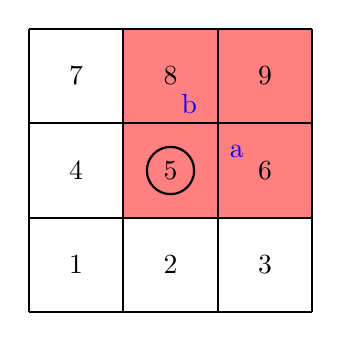
\begin{tikzpicture}[thick,scale=1.2,line join=round,>=latex]
  \fill[red!50, draw=none] (1,1) rectangle (3,3);
  
  \draw (1.5,1.5) circle (0.25);
  
  \foreach \i in {0,1,2,3} {
      \draw [color=black] (0,\i) -- (3,\i);
      \draw [color=black] (\i,0) -- (\i,3);
    }
  
  \draw (0.5, 0.5) node{$1$};
  \draw (1.5, 0.5) node{$2$};
  \draw (2.5, 0.5) node{$3$};
  \draw (0.5, 1.5) node{$4$};
  \draw (1.5, 1.5) node{$5$};
  \draw (2.5, 1.5) node{$6$};
  \draw (0.5, 2.5) node{$7$};
  \draw (1.5, 2.5) node{$8$};
  \draw (2.5, 2.5) node{$9$};
  
  \draw [color=blue] (2, 1.7) node{$\bigtimes$}; \draw [color=blue] (2.2, 1.7) node {a};
  \draw [color=blue] (1.7, 2) node{$\bigtimes$}; \draw [color=blue] (1.7, 2.2) node {b};
\end{tikzpicture}
\end{document}